%% ============================================================
%% Paper01_ChildSponsorship_Short.tex
%% Condensed public presentation (7 slides)
%% International child sponsorship and higher education aspirations
%% Daniel Prudencio -- M Csapek SA -- Education Economics (2025)
%%
%% Compile: cd Slides
%%   TEXINPUTS=../Preambles:$TEXINPUTS xelatex -interaction=nonstopmode Paper01_ChildSponsorship_Short.tex
%%   BIBINPUTS=..:$BIBINPUTS bibtex Paper01_ChildSponsorship_Short
%%   TEXINPUTS=../Preambles:$TEXINPUTS xelatex -interaction=nonstopmode Paper01_ChildSponsorship_Short.tex
%%   TEXINPUTS=../Preambles:$TEXINPUTS xelatex -interaction=nonstopmode Paper01_ChildSponsorship_Short.tex
%% ============================================================
\documentclass[aspectratio=169, 10pt]{beamer}
%% ============================================================
%% header.tex -- Shared Beamer preamble for Research Portfolio
%% Compile with: XeLaTeX (3-pass + bibtex)
%% Colors match Quarto/emory-clean.scss for cross-format consistency
%% ============================================================

%% ---- Packages -----------------------------------------------
\usepackage{fontspec}           % XeLaTeX font loading
\usepackage{unicode-math}       % Unicode math support
\usepackage{amsmath, mathtools} % Math environments
\usepackage{booktabs}           % Publication-quality tables
\usepackage{multirow}           % Multi-row table cells
\usepackage{graphicx}           % Include figures
\usepackage{xcolor}             % Color definitions
\usepackage{tcolorbox}          % Colored boxes
\tcbuselibrary{skins, breakable}
\usepackage{natbib}             % Author-year citations
\usepackage{appendixnumberbeamer} % Appendix slides don't count in total
\usepackage{hyperref}           % Hyperlinks
\usepackage{tikz}               % Diagrams (if needed)

%% ---- Fonts --------------------------------------------------
%% Using TeX Gyre Heros (Helvetica-style, bundled with MiKTeX).
%% To switch to Source Sans Pro: install it, then swap the two blocks below.
\setmainfont{TeX Gyre Heros}
\setsansfont{TeX Gyre Heros}
% Alternative: uncomment below and comment above if Source Sans Pro is installed
% \setmainfont{Source Sans Pro}[BoldFont=Source Sans Pro SemiBold]
% \setsansfont{Source Sans Pro}[BoldFont=Source Sans Pro SemiBold]

%% ---- Colors (matching emory-clean.scss) ---------------------
\definecolor{navyblue}{HTML}{012169}
\definecolor{institutgold}{HTML}{2E75B6}   % steel blue (was gold #B9975B)
\definecolor{highlightyellow}{HTML}{F2A900}
\definecolor{lightbg}{HTML}{E8EDF5}
\definecolor{darkgray}{HTML}{1a1a1a}
\definecolor{medgray}{HTML}{555555}
\definecolor{lightgray}{HTML}{f8f9fa}
\definecolor{positivegreen}{HTML}{15803d}
\definecolor{negativered}{HTML}{b91c1c}

%% ---- Beamer Theme -------------------------------------------
\usetheme{default}
\usecolortheme{default}
\setbeamertemplate{navigation symbols}{}   % No navigation clutter

%% Frame title
\setbeamercolor{frametitle}{fg=white, bg=navyblue}
\setbeamertemplate{frametitle}{%
  \vspace*{0.3em}%
  \insertframetitle%
  \vspace*{0.3em}%
}
\setbeamerfont{frametitle}{series=\bfseries, size=\large}

%% Title page colors
\setbeamercolor{title}{fg=navyblue}
\setbeamercolor{subtitle}{fg=institutgold}
\setbeamercolor{author}{fg=navyblue}
\setbeamercolor{institute}{fg=medgray}
\setbeamercolor{date}{fg=institutgold}

%% Body
\setbeamercolor{background canvas}{bg=white}
\setbeamercolor{normal text}{fg=darkgray}
\setbeamerfont{normal text}{family=\sffamily}

%% Itemize bullets
\setbeamercolor{item}{fg=navyblue}
\setbeamercolor{subitem}{fg=institutgold}
\setbeamertemplate{itemize item}{\small\textbullet}
\setbeamertemplate{itemize subitem}{\small$\rightarrow$}

%% Block environments
\setbeamercolor{block title}{fg=white, bg=navyblue}
\setbeamercolor{block body}{fg=darkgray, bg=lightbg}
\setbeamercolor{block title alerted}{fg=white, bg=institutgold}
\setbeamercolor{block body alerted}{fg=darkgray, bg=white}

%% Footer
\setbeamertemplate{footline}{%
  \hfill%
  \usebeamerfont{page number in head/foot}%
  \usebeamercolor[fg]{page number in head/foot}%
  \insertframenumber\,/\,\inserttotalframenumber\kern1em%
  \vskip4pt%
}
\setbeamercolor{page number in head/foot}{fg=medgray}

%% Section slides (automatically centered, navy bg)
\AtBeginSection[]{%
  \begin{frame}[plain]
    \begin{tikzpicture}[remember picture, overlay]
      \fill[navyblue] (current page.south west) rectangle (current page.north east);
      \node[white, font=\bfseries\Large, align=center] at (current page.center)
        {\insertsectionhead};
    \end{tikzpicture}
  \end{frame}%
}

%% ---- Custom Box Environments --------------------------------

%% keybox: gold background, for key takeaways
\newtcolorbox{keybox}{%
  colback=institutgold!12!white,
  colframe=institutgold,
  leftrule=4pt, rightrule=0pt, toprule=0pt, bottomrule=0pt,
  arc=4pt, outer arc=4pt,
  boxsep=2pt, left=6pt, right=6pt, top=5pt, bottom=5pt,
}

%% methodbox: navy left bar, for model/identification
\newtcolorbox{methodbox}{%
  colback=navyblue!5!white,
  colframe=navyblue,
  leftrule=4pt, rightrule=0pt, toprule=0pt, bottomrule=0pt,
  arc=4pt, outer arc=4pt,
  boxsep=2pt, left=6pt, right=6pt, top=5pt, bottom=5pt,
}

%% resultbox: gold border, for main findings
\newtcolorbox{resultbox}{%
  colback=institutgold!10!white,
  colframe=institutgold,
  leftrule=2pt, rightrule=2pt, toprule=2pt, bottomrule=2pt,
  arc=4pt, outer arc=4pt,
  boxsep=2pt, left=6pt, right=6pt, top=5pt, bottom=5pt,
}

%% assumptionbox: titled, formal assumptions
\newtcolorbox{assumptionbox}[1][]{%
  colback=highlightyellow!8!white,
  colframe=highlightyellow!70!black,
  leftrule=2pt, rightrule=2pt, toprule=2pt, bottomrule=2pt,
  arc=4pt, outer arc=4pt,
  boxsep=2pt, left=6pt, right=6pt, top=5pt, bottom=5pt,
  title={#1},
  fonttitle=\bfseries\small,
  attach boxed title to top left={yshift=-2mm, xshift=6pt},
  boxed title style={colback=highlightyellow!70!black, arc=2pt},
}

%% ---- Convenience Commands -----------------------------------
\newcommand{\gold}[1]{{\color{institutgold}\textbf{#1}}}
\newcommand{\navy}[1]{{\color{navyblue}\textbf{#1}}}
\newcommand{\pos}[1]{{\color{positivegreen}\textbf{#1}}}
\newcommand{\bad}[1]{{\color{negativered}\textbf{#1}}}   % red annotation
\newcommand{\hi}[1]{{\color{navyblue}\textbf{#1}}}
% Note: \alert is Beamer built-in (styled gold via alerted text color below)
\setbeamercolor{alerted text}{fg=institutgold}

%% ---- Math shortcuts -----------------------------------------
\newcommand{\E}{\mathbb{E}}
\newcommand{\Prob}{\mathbb{P}}
\newcommand{\ATE}{\mathrm{ATE}}
\newcommand{\ATT}{\mathrm{ATT}}
\newcommand{\MTE}{\mathrm{MTE}}
\newcommand{\Norm}{\mathcal{N}}


%% ---- TikZ libraries for DAG ---------------------------------
\usetikzlibrary{arrows.meta, positioning, calc}

%% ---- Bibliography -------------------------------------------
\bibliographystyle{aer}
\setcitestyle{authoryear, open={(}, close={)}}

%% ============================================================
\begin{document}

%% ---- 1. Title Slide -----------------------------------------
\begin{frame}[plain]
  \vspace{1.5em}
  \begin{center}
    {\color{navyblue}\Large\bfseries
      International Child Sponsorship Impact on the Intended\\[0.3em]
      Choice of Acquiring a Higher Education Degree:\\[0.3em]
      The Case of Rural Mexico}\\[1em]
    {\color{institutgold}\large\itshape Education Economics (2025)}\\[1.5em]
    {\color{navyblue}\normalsize\bfseries Daniel Prudencio}\\[0.3em]
    {\color{medgray}\small M Csapek SA \,/\, Tecnológico de Monterrey}\\[1.5em]
    {\color{institutgold}\small Published online: 17 May 2025}
  \end{center}
\end{frame}

%% ---- 2. The Puzzle ------------------------------------------
\begin{frame}{The Puzzle: Why Doesn't Education Pay Off Here?}
  \begin{columns}
    \begin{column}{0.60\textwidth}
      \textbf{The gap:} Returns to education are positive — yet \gold{educational attainment stays very low}
      \begin{itemize}
        \item Adults in Oaxaca and Chiapas average only \textbf{7.5 and 7.2 years} of schooling — barely above primary
        \item Both regions among the poorest in Mexico
      \end{itemize}
      \vspace{0.5em}
      \textbf{Standard explanation:} \bad{external constraints} — poverty, distance to schools, poor health\\[0.4em]
      \textbf{But also:} Growing evidence that \gold{internal constraints} matter too
      \begin{itemize}
        \item Aspirations, self-efficacy, and self-esteem shape whether children \textit{want} to pursue education
        \citep{Cunha2009, Dalton2016, Heckman2012}
      \end{itemize}
    \end{column}
    \begin{column}{0.36\textwidth}
      \begin{methodbox}
        \textbf{Research question:}\\[0.3em]
        Can an international child sponsorship program shift \textit{the level of education} children aspire to reach?
      \end{methodbox}
      \vspace{0.4em}
      \begin{keybox}
        \small \textbf{Compassion International (CI):} Third-largest child sponsorship program worldwide\\[0.2em]
        $\approx$\textbf{2.2 million} children across \textbf{29 countries}\\
        In Mexico: \textbf{33,360} children in $>$185 centers
      \end{keybox}
    \end{column}
  \end{columns}
\end{frame}

%% ---- 3. The Program and the Study ---------------------------
\begin{frame}{What Does CI Do? And How Do We Study It?}
  \begin{columns}
    \begin{column}{0.50\textwidth}
      \textbf{Three program pillars:}
      \begin{enumerate}
        \item \gold{Material support} — school supplies, uniforms, food, healthcare
        \item \gold{After-school program} — 5--6 hrs/week of academic tutoring and socio-emotional development (self-esteem, self-efficacy, life skills)
        \item \gold{Letter exchanges} with international sponsors — broadens career horizons and life possibilities
      \end{enumerate}
      \vspace{0.4em}
      Average \textbf{9.3 years} of participation\\
      \textit{De facto}: school attendance required for continued sponsorship
    \end{column}
    \begin{column}{0.47\textwidth}
      \begin{methodbox}
        \textbf{The study:}\\[0.2em]
        \begin{itemize}
          \item 2017 survey, \textbf{Oaxaca and Chiapas}, Mexico
          \item \textbf{8 rural communities}: 4 with CI, 4 matched controls
          \item \textbf{403 children aged 12--15} (163 sponsored, 240 non-sponsored)
          \item Key outcome: Does the child \textit{aspire} to a higher education degree?
        \end{itemize}
      \end{methodbox}
    \end{column}
  \end{columns}
\end{frame}


%% ---- 4. Identification Strategy -----------------------------
\begin{frame}{How Do We Measure CI's Causal Impact?}
  \begin{columns}
    \begin{column}{0.52\textwidth}
      \textbf{The challenge:} CI deliberately targets the \bad{poorest} children — sponsored and non-sponsored kids differ in ways we cannot fully measure
      \begin{itemize}
        \item Raw comparison of aspirations = \bad{not causal}
      \end{itemize}

      \vspace{0.1em}
      \textbf{The solution:} A \navy{binary Roy model} \citep{Aakvik2005}
      \begin{itemize}
        \item \gold{Instrument ($Z$):} Age when CI arrived in the village — younger children more likely selected, but age-at-arrival should not affect current aspirations
      \end{itemize}

      \vspace{0.4em}
      Identifies \navy{ATE} (average child), \navy{ATT} (sponsored), \navy{MTE} (by disadvantage)
    \end{column}
    \begin{column}{0.44\textwidth}
      \begin{center}
      \resizebox{0.92\columnwidth}{!}{%
      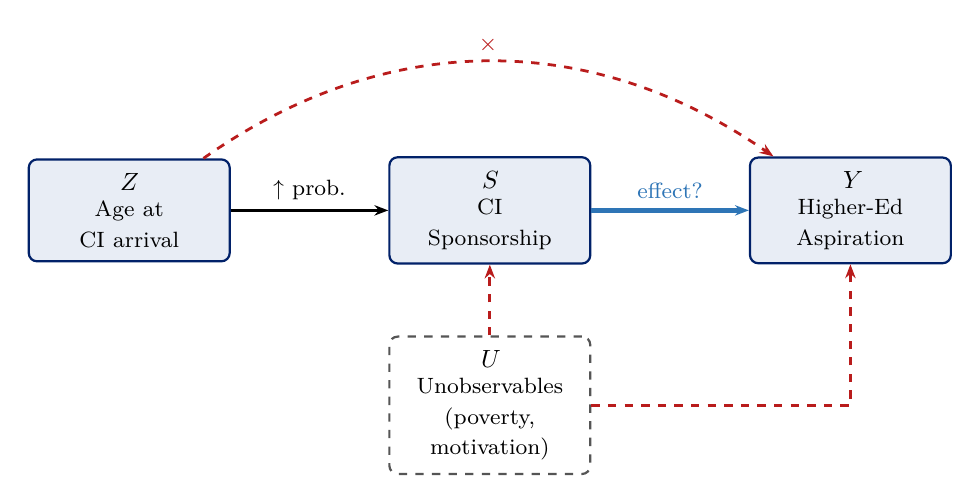
\begin{tikzpicture}[
          node distance = 1.4cm and 2.0cm,
          every node/.style = {font=\small},
          box/.style = {draw=navyblue, rounded corners=3pt, fill=lightbg,
                        inner sep=5pt, text width=2.2cm, align=center,
                        line width=0.8pt},
          latent/.style = {draw=medgray, rounded corners=3pt, fill=white,
                           inner sep=5pt, text width=2.2cm, align=center,
                           line width=0.8pt, dashed},
          arr/.style = {-{Stealth[length=5pt]}, line width=1pt},
          redarr/.style = {-{Stealth[length=5pt]}, dashed, negativered, line width=1pt},
          goldarr/.style = {-{Stealth[length=5pt]}, institutgold, line width=1.6pt},
        ]
        %% Nodes
        \node[box]  (Z) {$Z$\\\footnotesize Age at\\CI arrival};
        \node[box, right=of Z] (S) {$S$\\\footnotesize CI\\Sponsorship};
        \node[box, right=of S] (Y) {$Y$\\\footnotesize Higher-Ed\\Aspiration};
        \node[latent, below=0.9cm of S] (U) {$U$\\\footnotesize Unobservables\\(poverty, motivation)};

        %% Main arrows
        \draw[arr]    (Z) -- node[above, font=\footnotesize] {$\uparrow$ prob.} (S);
        \draw[goldarr](S) -- node[above, font=\footnotesize, institutgold] {effect?} (Y);

        %% Bias arrows
        \draw[redarr] (U) -- (S);
        \draw[redarr] (U) -| (Y);

        %% Excluded path Z -> Y (curved, red, with ×)
        \draw[redarr, bend left=35] (Z) to node[above, font=\footnotesize, negativered] {\texttimes} (Y);
      \end{tikzpicture}}% end resizebox
      \end{center}
      \vspace{0.2em}
      {\footnotesize\color{medgray} The Roy model corrects for $U$ by exploiting variation in $Z$\\
      \textcolor{negativered}{$\times$} = exclusion restriction: $Z$ does not directly affect aspirations}
    \end{column}
  \end{columns}
\end{frame}

%% ---- 5. Main Result -----------------------------------------
\begin{frame}{Main Result: CI Raises Aspirations}
  \begin{columns}
    \begin{column}{0.55\textwidth}
      \textbf{Effect on \textit{sponsored} children (ATT):}
      \begin{itemize}
        \item Estimated \gold{+17 to +20 percentage point} increase in the probability of aspiring to higher education
        \item Direction consistent with prior CI studies on adult outcomes \citep{Wydick2013}
      \end{itemize}
      \vspace{0.5em}
      \textbf{Statistical precision:}
      \begin{itemize}
        \item \bad{Not statistically significant} — small sample ($N=163$ sponsored) combined with a complex estimation model amplify uncertainty
        \item Results are \textit{suggestive}, not definitive — but the direction is clear and meaningful
      \end{itemize}
    \end{column}
    \begin{column}{0.41\textwidth}
      \begin{resultbox}
        \textbf{Back-of-envelope:}\\[0.4em]
        If higher aspirations translate into behavior, a \gold{20 pp increase} implies\\[0.3em]
        $\approx$ \textbf{8 more months of schooling}\\[0.3em]
        Consistent with \citet{Wydick2013}: 1.0--1.5 additional years of education for adult CI participants
      \end{resultbox}
      \vspace{0.4em}
      \begin{keybox}
        \small Even an imprecise result is informative: the program appears to be working in the right direction
      \end{keybox}
    \end{column}
  \end{columns}
\end{frame}

%% ---- 6. Two Additional Insights ----------------------------
\begin{frame}{Two Additional Insights}
  \begin{columns}
    \begin{column}{0.48\textwidth}
      \textbf{\navy{Insight 1:} CI's targeting is efficient}\\[0.4em]
      The Marginal Treatment Effect (MTE) shows that children \gold{most likely to be selected} into CI are also those who \gold{benefit the most} from it
      \begin{resultbox}
        \small \textbf{No efficiency-equity trade-off:} Aid programs often face a dilemma — targeting the most vulnerable may not reach those with the highest gains. \pos{CI avoids this dilemma:} the most disadvantaged children extract the greatest benefit
      \end{resultbox}
    \end{column}
    \begin{column}{0.48\textwidth}
      \textbf{\navy{Insight 2:} A surprising gender gap}\\[0.4em]
      \begin{itemize}
        \item \gold{Girls aspire more} to higher education than boys (boys are $\approx$12 pp less likely to aspire, among non-sponsored)
        \item Yet girls expect \bad{$\approx$50\% lower income} than boys at the same education level
      \end{itemize}
      \begin{keybox}
        \small The gender gap in aspirations is \textbf{not} explained by income beliefs — structural barriers and identity formation dominate at ages 12--15\\[0.3em]
        Information campaigns about female earnings alone are unlikely to close the gap
      \end{keybox}
    \end{column}
  \end{columns}
\end{frame}

%% ---- 7. Conclusions and Implications -----------------------
\begin{frame}{Conclusions and What It Means}
  \begin{columns}
    \begin{column}{0.50\textwidth}
      \textbf{What we found:}
      \begin{enumerate}
        \item CI has a \navy{positive, economically meaningful effect} on aspirations for higher education (ATT $\approx$17--20 pp) — suggestive, not conclusive
        \item CI's targeting is \navy{efficient}: the most vulnerable children benefit the most — no equity-efficiency trade-off
        \item \navy{Girls aspire more than boys} despite expecting much lower earnings — the gap is not explained by beliefs about future income
      \end{enumerate}
    \end{column}
    \begin{column}{0.47\textwidth}
      \textbf{What it means:}
      \begin{keybox}
        \small Holistic programs that \gold{combine material support with socio-emotional development} are well-positioned to shift aspirations — not just economic constraints
      \end{keybox}
      \vspace{0.4em}
      \begin{itemize}
        \item \gold{Informal attendance requirements} may be a valuable design feature — more time in school strengthens educational identity
        \item Intervening \gold{early (ages 9--12)} may be more effective than waiting for aspirations to be fully formed
        \item Gender-specific barriers require \gold{targeted interventions} beyond information provision
      \end{itemize}
    \end{column}
  \end{columns}
\end{frame}

%% ---- Bibliography -------------------------------------------
\begin{frame}[allowframebreaks]{References}
  \small
  \bibliography{../Bibliography_base}
\end{frame}

\end{document}
